\chapter{Estudo de caso: Sistema para detecção e supressão de incêndio}

O estudo de caso proposto é baseado no trabalho desenvolvido por~\citeauthor{kang2017room}, no qual um servidor MQTT para uma aplicação de IoT foi construído utilizando recursos do \textit{Amazon Web Services} (AWS). Para o presente estudo, será considerado apenas o módulo de detecção e supressão de incêndio elaborado por~\citeauthor{kang2017room}.

O sistema conta com quatro elementos principais: um servidor MQTT, chamado de \textit{Broker}; um aplicativo móvel; um detector de incêndio; e um chuveiro de combate à incêndios, também chamado de \textit{sprinkler}. No cenário descrito por~\citeauthor{kang2017room}, o usuário pode checar o status do \textit{sprinkler} (ligado/desligado) por meio do aplicativo, o qual emite uma mensagem de requisição de status para o \textit{sprinkler}, que responde logo em seguida. Quando as chamas são detectadas pelo sensor de incêndio, uma mensagem de alerta é enviada para o aplicativo e para o \textit{sprinker}, que é imediatamente acionado. Se, por alguma razão, o \textit{sprinkler} não for ativado, o usuário é notificado, e pode acioná-lo pelo aplicativo.

A Tabela~\ref{tab:iot_protocol} apresenta o conjunto de mensagens trocadas durante a execução do sistema, de acordo com a estratégia publicação/assinatura do protocolo MQTT. Para cada mensagem, um tópico de assinatura é fornecido, assim como o \textit{publisher} e o \textit{subscriber} envolvidos, isto é, aquele que envia e aquele que recebe a mensagem. Por fim, após cada mensagem recebida, uma ação é efetuada pelo \textit{subscriber}.

\begin{table}[!ht]
	\centering\tiny{
	\caption{Protocolo de troca de mensagens para a aplicação IoT sobre o MQTT~\cite{kang2017room}, adaptada pelo autor.}
	\label{tab:iot_protocol}
\begin{tabular}{|c|c|c|c|c|}
	\hline
	\rowcolor[HTML]{C0C0C0} 
	{\color[HTML]{000000} \textbf{Mensagem}}                             & {\color[HTML]{000000} \textbf{Tópico MQTT}} & {\color[HTML]{000000} \textit{\textbf{Publisher}}} & {\color[HTML]{000000} \textit{\textbf{Subscriber}}} & {\color[HTML]{000000} \textbf{Ação do \textit{subscriber}}} \\ \hline
	\textit{\begin{tabular}[c]{@{}c@{}}Fire\\ Detection\end{tabular}}    & \textit{Fire/Detected}                      & Sensor de incêndio                                 & \textit{App}                                        & Exibir notificação                                 \\ \hline
	\textit{\begin{tabular}[c]{@{}c@{}}Sprinkler\\ Request\end{tabular}} & \textit{Sprinkler/StReq}                    & \textit{App}                                       & \textit{Sprinkler}                                  & Ler status                                         \\ \hline
	\textit{\begin{tabular}[c]{@{}c@{}}Sprinkler\\ Reply\end{tabular}}   & \textit{Sprinkler/StRep}                    & \textit{Sprinkler}                                 & \textit{App}                                        & Enviar mensagem                                    \\ \hline
	\textit{\begin{tabular}[c]{@{}c@{}}Sprinkler\\ Start\end{tabular}}   & \textit{Sprinkler/Start}                    & \textit{App}                                       & \textit{Sprinkler}                                  & Ativar \textit{sprinkler}                                   \\ \hline
	\textit{\begin{tabular}[c]{@{}c@{}}Sprinkler\\ Start\end{tabular}}   & \textit{Sprinkler/Start}                    & Sensor de incêndio                                 & \textit{Sprinkler}                                  & Ativar \textit{sprinkler}                                  \\ \hline
\end{tabular}
	}
\end{table}

É importante ressalvar que, para receber uma mensagem, os agentes envolvidos devem estar previamente registrados no tópico correspondente. Esta característica do protocolo MQTT fica evidente na Figura~\ref{fig:estudo_msg}, na qual é apresentado um diagrama de sequência da troca de mensagens que representa o comportamento operacional do sistema.

\begin{figure}[ht]
	\centering
	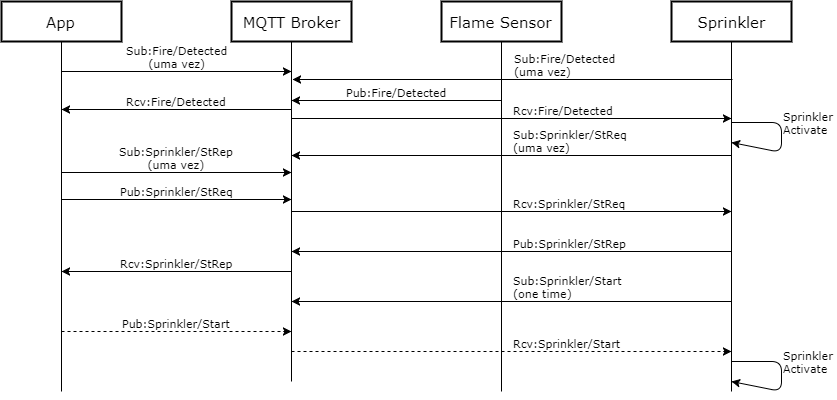
\includegraphics[width=1\textwidth]{imagens/projeto_msg.png}
	\caption{Procedimento de troca de mensagens do sistema IoT~\cite{kang2017room}, adaptado pelo autor.
		\label{fig:estudo_msg}}
\end{figure}
\FloatBarrier

Alguns elementos foram acrescentados na Figura~\ref{fig:estudo_msg} e na Tabela~\ref{tab:iot_protocol}, com a finalidade de deixá-las de acordo com as especificações do projeto. Ao descrever o cenário do aplicação,~\citeauthor{kang2017room} relatam que: "\textit{When the flame sensor detects the fire, the IoT device automatically alarms the fire event, activates the sprinkler to suppress the fire, and sends fire alarm message to smartphone app via IoT platform}". 

Observa-se que, os autores não deixam claro que o disparo do evento para ativação \textit{sprinkler} acontece mediante o recebimento de uma mensagem, que no caso, deve ser enviada pelo sensor de incêndio sob o tópico \textit{"Fire/Detected"}. 

Tanto na descrição do cenário quanto nos esquemas apresentados na Figura~\ref{fig:estudo_msg} e na Tabela~\ref{tab:iot_protocol}, o envio da mensagem de alerta de incêndio do sensor para o \textit{sprinkler} não é especificado. Sendo assim, foram adicionados procedimento para assinatura do tópico "\textit{Fire/Detected}" e recebimento do alerta por meio do tópico na Figura~\ref{fig:estudo_msg}, e a descrição do envio da mensagem na Tabela~\ref{tab:iot_protocol}.

Com base na descrição e objetivos do sistema, três processos que caracterizam seus compromissos são identificados: Detecção/Alerta; Checagem; e Supressão. Adiante, cada processo é modelado por meio da TPi de acordo com o comportamento operacional do MQTT quando QoS$=0$ e convertido em contrato multilateral por meio do algoritmo descrito na Seção~\ref{sec:algoritmo}. Por fim, o grafo de compromissos do sistema completo é obtido.

\section{Processo 1: Detecção/Alerta}

O processo de detecção e alerta de incêndio requer o envolvimento do sensor de incêndio, do \textit{Broker}, do aplicativo e do \textit{sprinkler}. Seu modelo em TPi é descrito como segue:
\begin{align}
& Sensor(FireDetection)~|~Broker()~|~App()~|~Sprinkler(),~em~que: \nonumber \\
& Sensor(z) \stackrel{def}{=} \overline{fd}\langle z \rangle \nonumber \\
& Broker() \stackrel{def}{=} fd(x).\overline{fd'}\langle x \rangle \nonumber \\
& App() \stackrel{def}{=} fd'(y) \nonumber \\
& Sprinkler() \stackrel{def}{=} fd'(y')
\end{align}

\subsection*{Aplicação do algoritmo}

O resultado obtido após a aplicação de cada passo do algoritmo é descrito como segue:
\begin{enumerate}
	\item $name$ = $C\_detectarIncêndio$;
	\item $Pi = (Sensor, FireDetection)$;
	\item $\mathcal{P} = \{Sensor, Broker, App, Sprinkler\}$;
	\item $\mathcal{D} = \{(Sensor, \{\overline{fd}\langle z \rangle\}), (Broker, \{fd(x).\overline{fd'}\langle x \rangle\}), (App, \{fd'(y)\}), (Sprinkler, \{fd'(y')\})\}$
	\item $\mathcal{A} = \{(\overline{fd}\langle z \rangle, Sensor), (fd(x), Broker), (\overline{fd'}\langle x \rangle, Broker), (fd'(y), App), (fd'(y'), Sprinkler)\}$
\end{enumerate}

De acordo com as regras estabelecidas na Seção~\ref{sec:algoritmo}, o compromisso pode ser declarado como:
\begin{eqnarray}
c_{1} = (C\_detectarIncendio, Sensor, Sprinkler, 5, \{&(\overline{fd}\langle z \rangle, tr), (fd(x), fi), (\overline{fd'}\langle x \rangle, tr), & \nonumber \\ &(fd'(y), fi), (fd'(y'), fi) \}) &
\end{eqnarray}

\section{Processo 2: Checagem}

O processo de checagem do status do \textit{sprinkler} requer o envolvimento do aplicativo, do \textit{broker} e do \textit{sprinkler}. Seu modelo em TPi é descrito a seguir:
\begin{align}
& App(SprinklerRequest)~|~Broker()~|~Sprinkler(),~em~que: \nonumber \\
& App(z) \stackrel{def}{=} \overline{req}\langle z \rangle . rep'(y) \nonumber \\
& Broker() \stackrel{def}{=} req(x) . \overline{req'}\langle x \rangle . rep(x') . \overline{rep'}\langle x' \rangle \nonumber \\
& Sprinkler() \stackrel{def}{=} req'(v) . \overline{rep}\langle reqReply \rangle
\end{align}

\subsection*{Aplicação do algoritmo}

O resultado obtido após a aplicação do algoritmo é exposto a seguir:
%alterar o Pi de dentro do () na descrição do algoritmo
\begin{enumerate}
	\item $name = C\_detectarIncendio$;
	\item $Pi = (App, SprinklerRequest)$;
	\item $\mathcal{P} = \{App, Broker, Sprinkler\}$
	\item $\mathcal{D} = \{ (App, \{\overline{req}\langle z \rangle . rep'(y)\}), (Broker, \{req(x) . \overline{req'}\langle x \rangle . rep(x') . \overline{rep'}\langle x' \rangle\}),$ 
	\\
	$(Sprinkler, \{req'(v) . \overline{rep}\langle reqReply \rangle\}) \};$
	\item $\mathcal{A} = \{ (\overline{req}\langle z \rangle, App), (req(x), Broker), (\overline{req'}\langle x \rangle, Broker), (req'(v), Sprinkler),
	\\
	(\overline{rep}\langle reqReply \rangle, Sprinkler), (rep(x'), Broker), (\overline{rep'}\langle x' \rangle, Broker), (rep'(y), App) \}.$
\end{enumerate}

Deste modo, o compromisso é definido como:
\begin{eqnarray}
c_{2} = (C\_checarStatus, App, App, 8,\{& (\overline{req}\langle z \rangle, tr), (req(x), fi), (\overline{req'}\langle x \rangle, tr)& \nonumber \\ 
&(req'(v), fi), (\overline{rep}\langle reqReply \rangle, tr), (rep(x'), fi), & \nonumber \\ 
&(\overline{rep'}\langle x' \rangle, tr), (rep'(y), fi) \} )&
\end{eqnarray}

\section{Processo 3: Supressão}

O processo de supressão de incêndio requer o envolvimento do sensor de incêndio, do Broker, do App e do Sprinkler. Seu modelo em TPi pode ser descrito abaixo:

\begin{align}
&Sensor(FireDetection)~|~Broker()~|~App()~|Sprinkler(),~em~que: \nonumber \\
&Sensor(z) \stackrel{def}{=} \overline{fd}\langle z \rangle \nonumber \\
&Broker \stackrel{def}{=} fd(x) . \overline{fd'}\langle x \rangle .  st(x') . \overline{st'}\langle x' \rangle \nonumber \\
&App() \stackrel{def}{=} fd'(s) . \overline{st}\langle startSprinkler \rangle  \nonumber \\
&Sprinkler() \stackrel{def}{=} st'(y)
\end{align}

\subsection*{Aplicação do algoritmo}

O resultado atingido após a aplicação do algoritmo é descrito a seguir:
\begin{enumerate}
	\item $name = C\_suprirIncendio$;
	\item $Pi = (Sensor, FireDetection)$;
	\item $\mathcal{P} = \{Sensor, Broker, App, Sprinkler\}$;
	\item $\mathcal{D} = \{ (Sensor, \{ \overline{fd}\langle z \rangle \nonumber \}), 
	(Broker, \{  fd(x) . \overline{fd'}\langle x \rangle .  st(x') . \overline{st'}\langle x' \rangle  \}), 
	\\
	(App, \{ fd'(s) . \overline{st}\langle startSprinkler \rangle \}), 
	(Sprinkler, \{ st'(y) \}) \};$
	\item $\mathcal{A} = \{ (\overline{fd}\langle z \rangle, Sensor), (fd(x), Broker), (\overline{fd'}\langle x \rangle, Broker), (fd'(s), App), 
	\\
	(\overline{st}\langle startSprinkler \rangle, App), (st(x'), Broker), (\overline{st'}\langle x' \rangle, Broker), (st'(y), Sprinkler) \}.$
\end{enumerate}

Assim, o compromisso é definido como segue:
\begin{eqnarray}
c_{3} = \{ C\_suprirIncendio, Sensor, Sprinkler, 8, \{& (\overline{fd}\langle z \rangle, tr), (fd(x), fi), & \nonumber \\  &(\overline{fd'}\langle x \rangle, tr) 
(fd'(s), fi), & \nonumber \\ & (\overline{st}\langle startSprinkler \rangle, tr), (st(x'), fi), & \nonumber \\ & (\overline{st'}\langle x' \rangle, tr), (st'(y), fi) \}&
\end{eqnarray}